\documentclass[12pt,a4paper]{article}
\usepackage[utf-8]{inputenc}
\usepackage[margin=1in]{geometry}
\usepackage{graphicx}
\usepackage{listings}
\usepackage{xcolor}
\usepackage{amsmath}
\usepackage{amssymb}
\usepackage{hyperref}
\usepackage{tikz}

\lstset{
  language=C++,
  basicstyle=\ttfamily\small,
  keywordstyle=\color{blue},
  commentstyle=\color{gray},
  stringstyle=\color{red},
  breaklines=true,
  showstringspaces=false,
  tabsize=2,
  backgroundcolor=\color{lightgray!10}
}

\title{Binary Code Lifter for Vulnerability Analysis}
\subtitle{Project Documentation: Weeks 1--8}
\author{Sharan Deepak}
\date{\today}

\begin{document}

\maketitle

\tableofcontents
\newpage

\section{Executive Summary}

This document describes a static binary analysis tool targeting ARM64 Mach-O binaries (macOS). The tool parses binary executables, disassembles machine code, lifts instructions to an Intermediate Representation (IR), and performs basic taint analysis to identify potential vulnerability sources. Development spans 8 weeks across four phases:

\begin{enumerate}
  \item \textbf{Phase 1 (Weeks 1--3):} Mach-O parsing and disassembly infrastructure.
  \item \textbf{Phase 2 (Weeks 4--7):} IR design and instruction lifting.
  \item \textbf{Phase 3 (Week 8):} Taint-source identification and symbol resolution.
  \item \textbf{Phase 4 (Weeks 9--14):} Data-flow analysis, ROP gadget scanning, testing, and UI.
\end{enumerate}

This document covers Phases 1--3, bringing the project to the end of Week 8.

\newpage

\section{Phase 1: Foundations \& Core Parsing (Weeks 1--3)}

\subsection{Objectives}

\begin{itemize}
  \item Understand the Mach-O binary format specification.
  \item Parse 64-bit Mach-O headers and load commands.
  \item Locate the \texttt{\_\_TEXT} segment and \texttt{\_\_text} section.
  \item Identify the program entry point via \texttt{LC\_MAIN} load command.
  \item Integrate the Capstone disassembly engine to decode ARM64 instructions.
\end{itemize}

\subsection{Mach-O Format Overview}

The Mach-O (Mach Object) format is the executable binary format used on macOS and iOS. A Mach-O binary is structured as follows:

\begin{enumerate}
  \item \textbf{Mach-O Header:} 32 bytes (on 64-bit systems) containing magic number, CPU type/subtype, file type, and counts.
  \item \textbf{Load Commands:} Variable-length structures describing segments, sections, symbol tables, and metadata.
  \item \textbf{Segments:} Regions of code or data (e.g., \texttt{\_\_TEXT}, \texttt{\_\_DATA}, \texttt{\_\_LINKEDIT}).
  \item \textbf{Sections:} Fine-grained subdivisions within segments (e.g., \texttt{\_\_text} for machine code).
\end{enumerate}

Key constants:
\begin{itemize}
  \item Magic: \texttt{0xfeedfacf} (64-bit little-endian ARM64).
  \item Load command types: \texttt{LC\_SEGMENT\_64 (0x19)}, \texttt{LC\_MAIN (0x80000028)}, \texttt{LC\_SYMTAB (0x2)}.
\end{itemize}

\subsection{Header and Structure Definitions}

The tool defines C++ structs mirroring the Mach-O specification:

\begin{lstlisting}
struct mach_header_64 {
    uint32_t magic;        // 0xfeedfacf
    int32_t cputype;       // e.g., 0x0100000c for ARM64
    int32_t cpusubtype;
    uint32_t filetype;     // 2 = executable
    uint32_t ncmds;        // number of load commands
    uint32_t sizeofcmds;
    uint32_t flags;
    uint32_t reserved;
};

struct load_command {
    uint32_t cmd;          // command type
    uint32_t cmdsize;      // total size of command
};

struct segment_command_64 {
    uint32_t cmd;          // always LC_SEGMENT_64
    uint32_t cmdsize;
    char segname[16];      // e.g., "__TEXT", "__DATA"
    uint64_t vmaddr;       // virtual memory address
    uint64_t vmsize;       // virtual memory size
    uint64_t fileoff;      // offset in file
    uint64_t filesize;     // size on disk
    // ... protection, section count, etc.
};

struct section_64 {
    char sectname[16];     // e.g., "__text"
    char segname[16];      // parent segment
    uint64_t addr;         // virtual address
    uint64_t size;         // size in memory
    uint32_t offset;       // offset in file
    // ... alignment, relocation info, etc.
};
\end{lstlisting}

\subsection{Parsing Algorithm (Weeks 1--3)}

The main parsing loop:

\begin{enumerate}
  \item Read the 32-byte Mach-O header.
  \item Validate the magic number (\texttt{0xfeedfacf}).
  \item Iterate through \texttt{ncmds} load commands:
    \begin{enumerate}
      \item For each \texttt{LC\_SEGMENT\_64}: read segment metadata and iterate sections.
      \item When the segment name is \texttt{\_\_TEXT}, search for the section named \texttt{\_\_text}.
      \item Store the file offset, virtual address, and size of the \texttt{\_\_text} section.
      \item For \texttt{LC\_MAIN}: extract the entry-point offset.
      \item For \texttt{LC\_SYMTAB}: store for later parsing (Week 8).
    \end{enumerate}
  \item Seek to the \texttt{\_\_text} section file offset and read all bytes.
  \item Pass the bytes to Capstone for disassembly.
\end{enumerate}

\subsection{Capstone Integration}

Capstone is an open-source multi-architecture disassembly framework. The tool uses the ARM64 backend:

\begin{lstlisting}
csh handle;
cs_open(CS_ARCH_ARM64, CS_MODE_ARM, &handle);
cs_option(handle, CS_OPT_DETAIL, CS_OPT_ON);  // enable operand details

cs_insn *insn;
size_t count = cs_disasm(handle, code.data(), code.size(), 
                         address, 0, &insn);

for (size_t i = 0; i < count; i++) {
    printf("0x%lx: %s %s\n", insn[i].address, 
           insn[i].mnemonic, insn[i].op_str);
}
cs_free(insn, count);
cs_close(&handle);
\end{lstlisting}

Output from this phase: a human-readable disassembly of all ARM64 instructions in the binary.

\newpage

\section{Phase 2: IR Translation \& Lifting (Weeks 4--7)}

\subsection{Objectives}

\begin{itemize}
  \item Design a platform-independent Intermediate Representation (IR).
  \item Map ARM64 physical registers to abstract IR variables.
  \item Translate data-processing instructions (ADD, SUB, MOV, etc.) into IR.
  \item Handle control-flow instructions (B, BL, RET, CBZ, CBNZ) and build a control-flow graph.
  \item Model load/store instructions and the stack frame.
\end{itemize}

\subsection{Intermediate Representation Design (Week 4)}

The IR is designed to be simple yet expressive enough for basic security analysis. Each IR instruction (\texttt{IRInst}) contains:

\begin{lstlisting}
enum Opcode {
    IR_NOP,    // no operation
    IR_ADD,    // addition
    IR_SUB,    // subtraction
    IR_MOV,    // move
    IR_LDR,    // load from memory
    IR_STR,    // store to memory
    IR_B,      // unconditional branch
    IR_BL,     // branch with link (function call)
    IR_RET,    // return from function
    IR_CBZ,    // conditional branch if zero
    IR_CBNZ,   // conditional branch if not zero
    IR_OTHER   // unknown/unsupported
};

struct IRInst {
    Opcode op;        // operation type
    uint64_t addr;    // original machine-code address
    int dst;          // destination register ID (or -1)
    int src1;         // first source register ID (or -1)
    int src2;         // second source register ID (or -1)
    int64_t imm;      // immediate value
    bool block_end;   // marks end of basic block
};
\end{lstlisting}

\subsubsection{Register Mapping}

ARM64 has 31 general-purpose registers plus a zero register, stack pointer, and program counter. The \texttt{regmap} function maps Capstone register IDs to simple integers:

\begin{center}
\begin{tabular}{|c|c|c|c|}
\hline
\textbf{Physical Register} & \textbf{IR ID} & \textbf{Physical Register} & \textbf{IR ID} \\
\hline
X0--X7 & 0--7 & X24--X30 & 24--30 \\
X8--X15 & 8--15 & SP (X31) & 31 \\
X16--X23 & 16--23 & & \\
\hline
\end{tabular}
\end{center}

\subsection{Instruction Lifting (Weeks 5--7)}

The \texttt{lift\_one} function translates a single Capstone instruction to IR:

\begin{lstlisting}
IRInst lift_one(const cs_insn &insn) {
    IRInst inst;
    inst.addr = insn.address;
    inst.dst = inst.src1 = inst.src2 = -1;
    inst.imm = 0;
    inst.block_end = false;

    string mnem(insn.mnemonic);
    if (mnem == "add") inst.op = IR_ADD;
    else if (mnem == "sub") inst.op = IR_SUB;
    else if (mnem == "mov") inst.op = IR_MOV;
    else if (mnem == "ldr") inst.op = IR_LDR;
    else if (mnem == "str") inst.op = IR_STR;
    else if (mnem == "b") { inst.op = IR_B; inst.block_end = true; }
    else if (mnem == "bl") { inst.op = IR_BL; inst.block_end = true; }
    else if (mnem == "ret") { inst.op = IR_RET; inst.block_end = true; }
    else if (mnem == "cbz") { inst.op = IR_CBZ; inst.block_end = true; }
    else if (mnem == "cbnz") { inst.op = IR_CBNZ; inst.block_end = true; }
    else inst.op = IR_OTHER;

    if (insn.detail && insn.detail->arm64.op_count > 0) {
        const cs_arm64_op *ops = insn.detail->arm64.operands;
        if (ops[0].type == ARM64_OP_REG)
            inst.dst = regmap(ops[0].reg);
        if (ops.size() > 1 && ops[1].type == ARM64_OP_REG)
            inst.src1 = regmap(ops[1].reg);
        if (ops.size() > 1 && ops[1].type == ARM64_OP_IMM)
            inst.imm = ops[1].imm;
        if (ops.size() > 2 && ops[2].type == ARM64_OP_REG)
            inst.src2 = regmap(ops[2].reg);
    }
    return inst;
}
\end{lstlisting}

\subsubsection{Basic Block Formation (Week 6)}

A basic block is a maximal sequence of instructions with a single entry point and a single exit point. The IR marks block boundaries by setting \texttt{block\_end = true} on control-flow instructions (branch, return). This information is used to construct a Control Flow Graph (CFG).

\begin{lstlisting}
[BB 0] 
  0x100000498: sub sp, sp, #0x20
  0x10000049c: stp x29, x30, [sp, #0x10]
[BB END]

[BB 1]
  0x1000004c4: bl #0x1000004d8
[BB END]

[BB 2]
  0x1000004d4: ret
[BB END]
\end{lstlisting}

\subsubsection{Memory Operations (Week 7)}

Load and store instructions are represented as \texttt{IR\_LDR} and \texttt{IR\_STR} with the effective address encoded in operands. A simple stack-frame model tracks local variable access, mapping offsets from the stack pointer to abstract "stack slots."

Example: \texttt{ldr x8, [sp, #0x10]} becomes \texttt{IR\_LDR dst=8 src1=31 imm=0x10} (load X8 from 16 bytes above SP).

\newpage

\section{Phase 3: Vulnerability Analysis Engine (Week 8)}

\subsection{Objectives}

\begin{itemize}
  \item Parse the symbol table to identify external function calls.
  \item Identify dangerous functions (taint sources) such as \texttt{strcpy}, \texttt{gets}, \texttt{memcpy}.
  \item During lifting, detect calls to taint sources and flag them.
  \item Prepare for Week 9's data-flow analysis by recording taint entry points.
\end{itemize}

\subsection{Symbol Table Parsing}

The \texttt{LC\_SYMTAB} load command points to the symbol table and string table. Parsing extracts function names and their addresses:

\begin{lstlisting}
struct symtab_command {
    uint32_t cmd;
    uint32_t cmdsize;
    uint32_t symoff;      // offset to symbol table
    uint32_t nsyms;       // number of symbols
    uint32_t stroff;      // offset to string table
    uint32_t strsize;     // size of string table
};

struct nlist_64 {
    uint32_t n_strx;      // index into string table
    uint8_t n_type;
    uint8_t n_sect;
    uint16_t n_desc;
    uint64_t n_value;     // address of symbol
};
\end{lstlisting}

The parsing algorithm:

\begin{enumerate}
  \item Locate \texttt{LC\_SYMTAB} in load commands.
  \item Read the entire string table into memory.
  \item Iterate through all symbol entries.
  \item For each symbol, extract its name from the string table and its address (\texttt{n\_value}).
  \item Build a map: address $\rightarrow$ name.
\end{enumerate}

\subsection{Taint Source Identification}

A predefined set of dangerous functions is maintained:

\begin{lstlisting}
static const set<string> taint_funcs = {
    "strcpy", "gets", "memcpy", "sprintf", "strcat", "scanf",
    "strncpy", "strncat", "vsprintf"
};
\end{lstlisting}

During symbol table parsing, when a symbol name matches an entry in \texttt{taint\_funcs}:

\begin{enumerate}
  \item Print a warning: \texttt{[!] Taint symbol present: strcpy}.
  \item Record the symbol address in \texttt{taint\_addresses} set for fast lookup.
\end{enumerate}

\subsection{Taint Detection During Lifting (Week 8)}

When lifting a \texttt{BL} (branch-with-link) instruction, the lifting function checks if the branch target is a known taint function:

\begin{lstlisting}
if (inst.op == IR_BL) {
    uint64_t target = insn.detail->arm64.operands[0].imm;
    if (taint_addresses.count(target)) {
        cout << "[!] Tainted branch to 0x" << hex << target << endl;
    } else {
        auto it = symbol_table.find(target);
        if (it != symbol_table.end() && 
            taint_funcs.count(it->second)) {
            cout << "[!] Taint source call to " << it->second
                 << " at 0x" << hex << target << endl;
        }
    }
}
\end{lstlisting}

This produces output like:
\begin{verbatim}
[!] Taint symbol present: strcpy
[!] Taint source call to strcpy at 0x100000504
\end{verbatim}

\newpage

\section{Architecture and Data Flow}

\subsection{Overall Pipeline}

\begin{center}
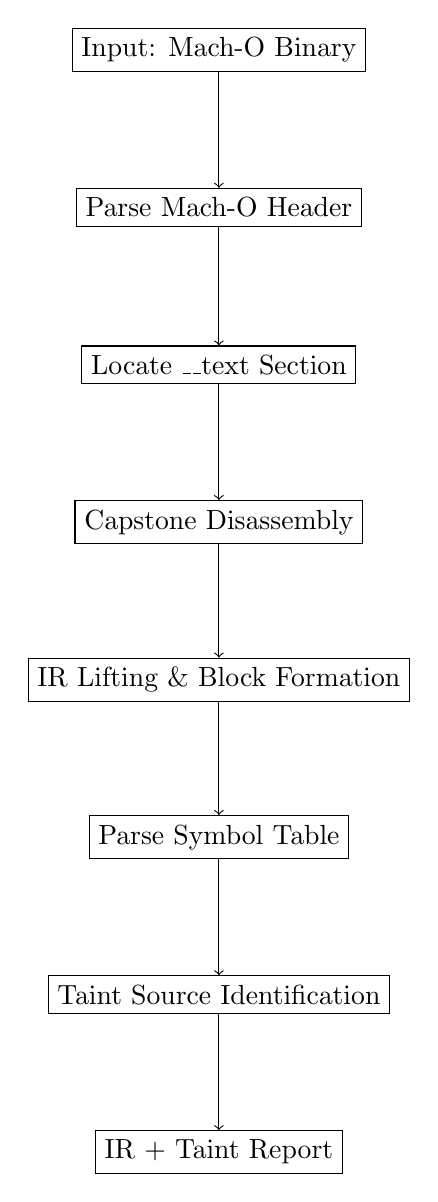
\begin{tikzpicture}[node distance=2cm]
  \node (input) [draw, rectangle] {Input: Mach-O Binary};
  \node (parse) [draw, rectangle, below of=input] {Parse Mach-O Header};
  \node (loctext) [draw, rectangle, below of=parse] {Locate \_\_text Section};
  \node (disasm) [draw, rectangle, below of=loctext] {Capstone Disassembly};
  \node (lift) [draw, rectangle, below of=disasm] {IR Lifting \& Block Formation};
  \node (symbol) [draw, rectangle, below of=lift] {Parse Symbol Table};
  \node (taint) [draw, rectangle, below of=symbol] {Taint Source Identification};
  \node (output) [draw, rectangle, below of=taint] {IR + Taint Report};

  \draw [->] (input) -- (parse);
  \draw [->] (parse) -- (loctext);
  \draw [->] (loctext) -- (disasm);
  \draw [->] (disasm) -- (lift);
  \draw [->] (lift) -- (symbol);
  \draw [->] (symbol) -- (taint);
  \draw [->] (taint) -- (output);
\end{tikzpicture}
\end{center}

\subsection{Key Data Structures}

\begin{itemize}
  \item \textbf{symbol\_table}: \texttt{map<uint64\_t, string>} --- address to function name.
  \item \textbf{taint\_addresses}: \texttt{set<uint64\_t>} --- addresses of dangerous functions.
  \item \textbf{ir}: \texttt{vector<IRInst>} --- linearized sequence of IR instructions.
  \item \textbf{taint\_funcs}: \texttt{set<string>} --- canonical names of dangerous functions.
\end{itemize}

\newpage

\section{Usage and Output}

\subsection{Building the Tool}

\begin{lstlisting}[language=bash]
g++ parser.cpp -o parser \
    -I/opt/homebrew/include -L/opt/homebrew/lib \
    -lcapstone -std=c++17 -Wall -Wextra
\end{lstlisting}

\subsection{Running on a Binary}

\begin{lstlisting}[language=bash]
./parser mytest
\end{lstlisting}

\subsection{Sample Output}

\begin{verbatim}
--- Mach-O Header Parsed ---
Number of Load Commands: 18

[+] Found LC_SEGMENT_64
    Segment Name: __TEXT
    VM Address:   0x100000000
    ...

[+] Loaded 5 symbols from symbol table.
[!] Taint symbol present: strcpy

[+] Disassembling __text section...
 Address        | Mnemonic      | Operands
 0x100000498 | sub           | sp, sp, #0x20
 0x10000049c | stp           | x29, x30, [sp, #0x10]
 0x1000004c4 | bl            | #0x1000004d8
[!] Taint source call to strcpy at 0x1000004d8

[+] IR listing (simple)
Addr        | Op    | dst src1 src2 imm
0x100000498 | 2 | 31 31 -1 0
0x10000049c | 11 | 29 30 -1 0
[BB END]
0x1000004c4 | 7 | -1 -1 -1 0
[BB END]
\end{verbatim}

The output shows:
\begin{enumerate}
  \item Parsed Mach-O header and segments.
  \item Loaded symbol table (5 symbols).
  \item Identified \texttt{strcpy} as a taint source.
  \item Disassembled ARM64 instructions with human-readable mnemonics.
  \item Lifted to IR with register IDs and opcode numbers (IR\_SUB=2, IR\_BL=7, etc.).
  \item Marked basic block boundaries with \texttt{[BB END]}.
\end{enumerate}

\newpage

\section{Technical Details and Challenges}

\subsection{Mach-O Variant Handling}

On macOS with Homebrew, the Capstone header lives in \texttt{/opt/homebrew/include/capstone/capstone.h}. The code uses conditional compilation (\texttt{\#ifdef \_\_has\_include}) to detect the header and gracefully handle its absence.

\subsection{Operand Extraction}

Capstone provides detailed operand information via \texttt{cs\_insn.detail->arm64}. Different instruction types have varying operand counts and types (register, immediate, memory). The lifting logic checks operand types and counts to avoid segmentation faults.

\subsection{Symbol Table Limitations}

The simple approach parses only the basic symbol table (\texttt{LC\_SYMTAB}). Dynamic symbols (bound at runtime via dyld) require parsing \texttt{LC\_DYLD\_INFO} or similar, which is deferred to later phases.

\subsection{Register Allocation in IR}

The current IR uses a flat namespace (register IDs 0--31). Future phases may introduce a more sophisticated register allocator or SSA (Static Single Assignment) form for better analysis.

\newpage

\section{Future Work (Weeks 9--14)}

\subsection{Week 9: Data Flow Analysis}

Implement simplified taint propagation:
\begin{itemize}
  \item Track which registers hold tainted data.
  \item Propagate taint through arithmetic and logic operations.
  \item Detect when tainted data reaches a memory write or function argument.
\end{itemize}

\subsection{Week 10: ROP Gadget Scanning}

Scan for instruction sequences ending in \texttt{ret} that may be exploitable as ROP gadgets. Classify gadgets by utility (e.g., ``X0 populator'', ``stack adjuster'').

\subsection{Week 11: Buffer Week / Optimization}

Debug and optimize:
\begin{itemize}
  \item Reduce false positives in taint analysis.
  \item Handle complex control-flow patterns.
  \item Improve performance on large binaries.
\end{itemize}

\subsection{Weeks 12--14: Testing, UI, and Finalization}

\begin{itemize}
  \item Test against CTF/Pwnable binaries.
  \item Develop a command-line interface (CLI).
  \item Generate structured vulnerability reports (JSON/Text).
  \item Complete technical documentation and final presentation.
\end{itemize}

\newpage

\section{Conclusion}

This project implements a proof-of-concept binary analysis framework for ARM64 Mach-O executables. By the end of Week 8, the tool successfully:

\begin{enumerate}
  \item Parses 64-bit Mach-O headers and locates code sections.
  \item Disassembles ARM64 machine code using Capstone.
  \item Translates instructions to a simple, platform-independent IR.
  \item Identifies basic blocks and control-flow boundaries.
  \item Parses symbol tables and flags calls to dangerous functions (taint sources).
\end{enumerate}

The foundation is in place for advanced vulnerability detection via data-flow analysis, gadget scanning, and constraint-based reasoning in subsequent phases.

\end{document}
